\section{Experiment}
A good model, especially facing with small sample segmentation, should generalize well instead of overfitting on a small number of training data. The whole point of data augmentation, adding noise, etc, is to improve the generalizability of the trained neural network so that for the unseen data, the model predict reasonably well.\\

Due to the limited ability of the GPU resource available, tuning hyper-parameters using grid search is too inefficient. Thus in our experiment, we leveraged the optimizer scheduler in PyTorch so that starting from the learning rate starts from $lr=2\times10^{-4}$ and decreased to 0.8 * lr every 25 epochs so that the learning rate approach 0 in the later training stage.  
\begin{enumerate}
	\item \textbf{learning rate}
	\item \textbf{Optimizer:} We used Adam optimizer considering that Model Genesis, winning solution for NSCLC segmentation as well as other well known solutions used the model optimizer.
	\item \textbf{Epochs:} The maximum number of epochs for training is 500. However, each epoch we validate the result and the best model was saved throughout the training process. We count the number of continued non-improving epochs, and when it reached 30 epochs, the training progress terminated automatically.
	\end{enumerate}

\section{With Fully labelled data}
We first consider training on a small dataset and all of them are labelled with segmentation masks, because this is the case during the first few months of this project when only 20 volumes of the Covid lungs from the Covid Segmentation benchmark were publicly available, later in July 2020, MosMed published a new dataset containing 50 labeled slices.

\subsection{Experiment Setup}
To fully leverage the Covid Dataset, we combined the 20 volumes in Covid Segmentation bechmark and the 50 volumes MosMed Dataset. We randomly selected 20 volumes for testing, and further split the 50 remaining volume into 5 fold for cross validation. Smaller sample: One fold (10 volumes) for training; Normal training: Four fold (40 Volumes) for training.
Note that since we cannot do anything to the various slice thickness, we sliced the volume into 2D.

\subsection{Best results}
For the segmentation of infection area using \textbf{fully labelled sample only}, we achieved Dice score (DSC) on the training set (50 volumes sliced in 2D) of 99.0321\%, 80.3601\% on the validation set and 79.9356\% on the testing set. All the volumes was preprocessed as described in Section 3 and augmented the data using random rotating, and elastic transformation and {\color{red}mix up augmentation} on the training set only.

\subsection{Training}
We compared the model trained from scratch and with transfer learning in this experiment. More specifically, we experimented two transfer learning intialization in this section. First we trained the Binary segmentation task with the images from NSCLC and MSD dataset, then the model was fine tuned using two different methods suggested in work \cite{wang_improving_2019}: Fine-Tuning all layers (reinitialize the last layer), and Fine-Tuning only the Decoder, shown in figure \ref{fig:transfer-learning-graph}.\\

%\begin{figure}
%	\centering
%	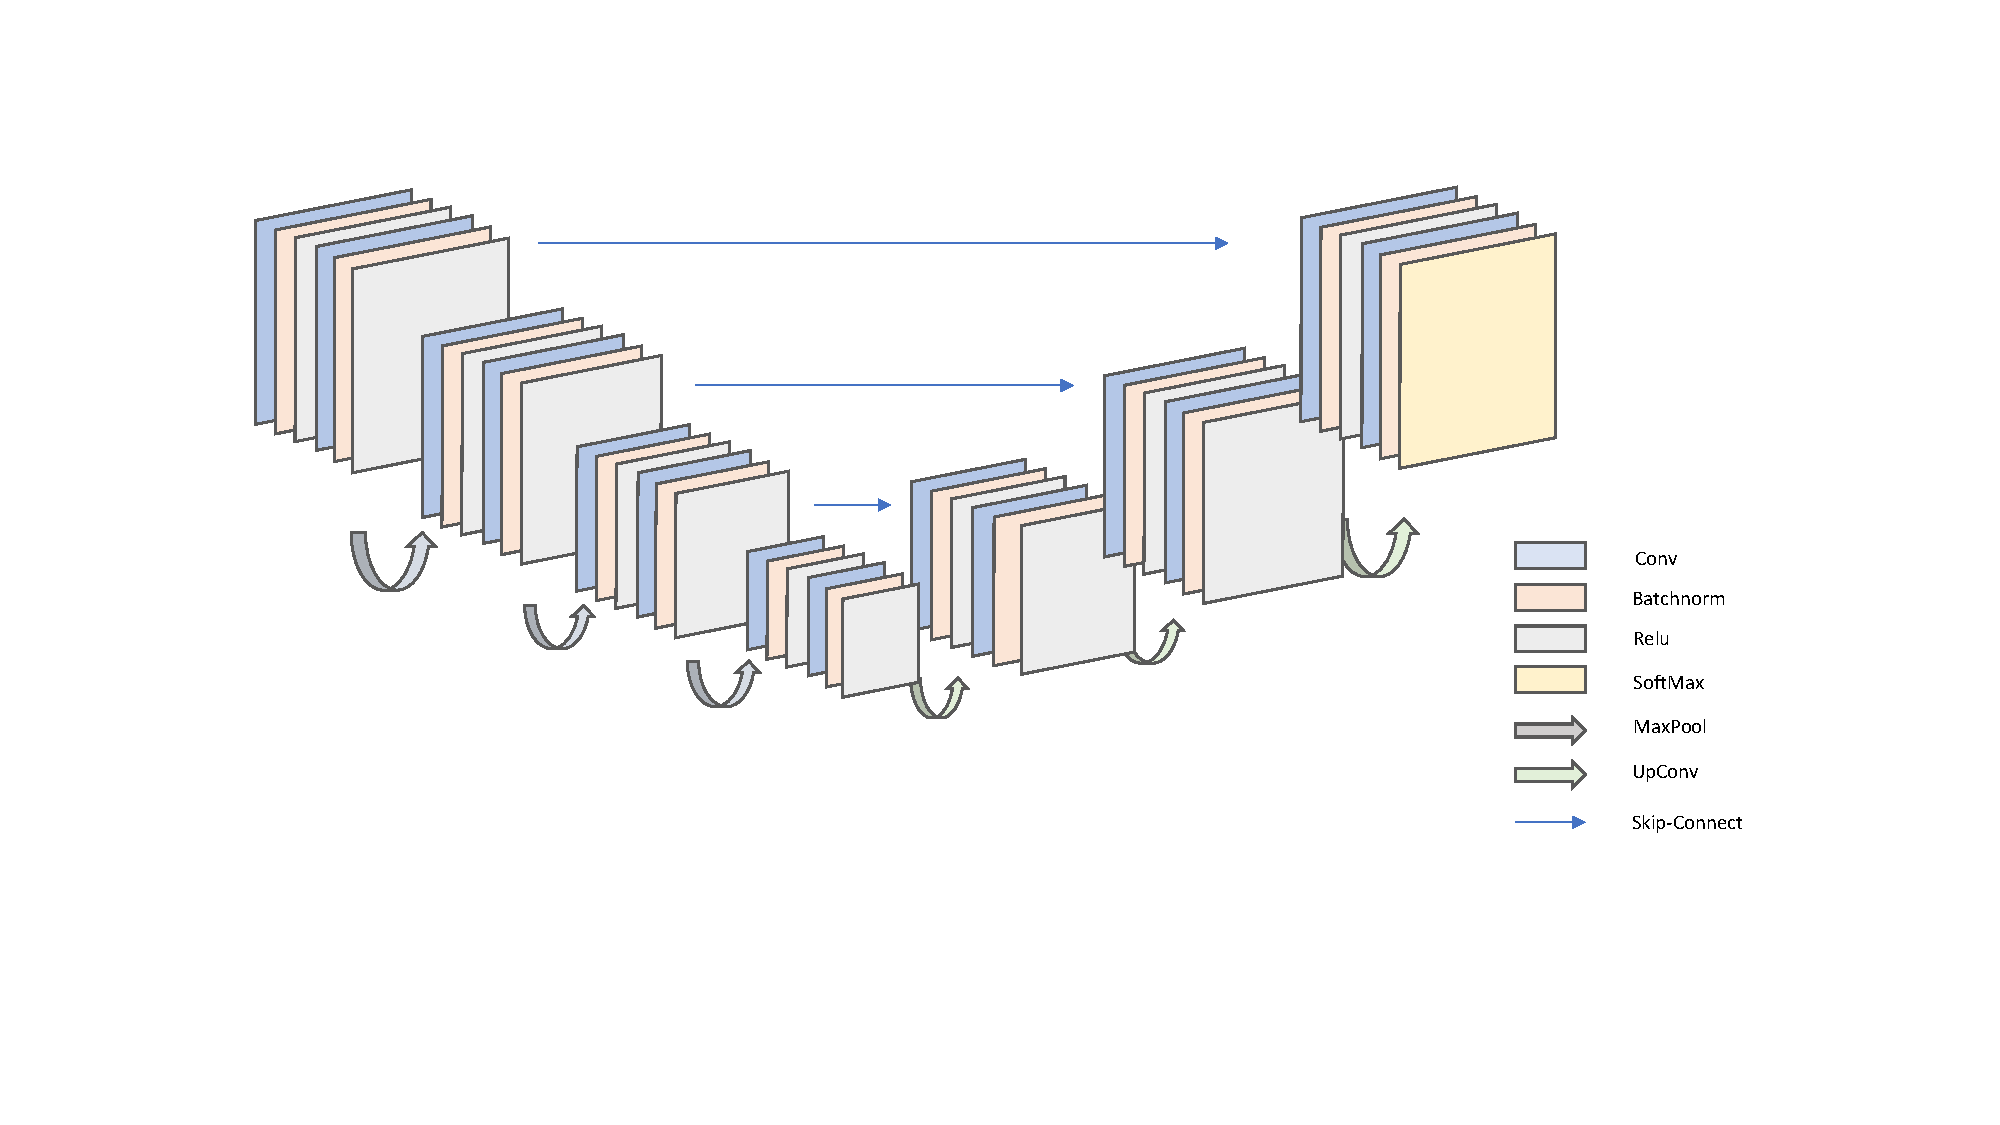
\includegraphics[width=0.8\textwidth]{img/Networks/Unet-train.pdf}
%	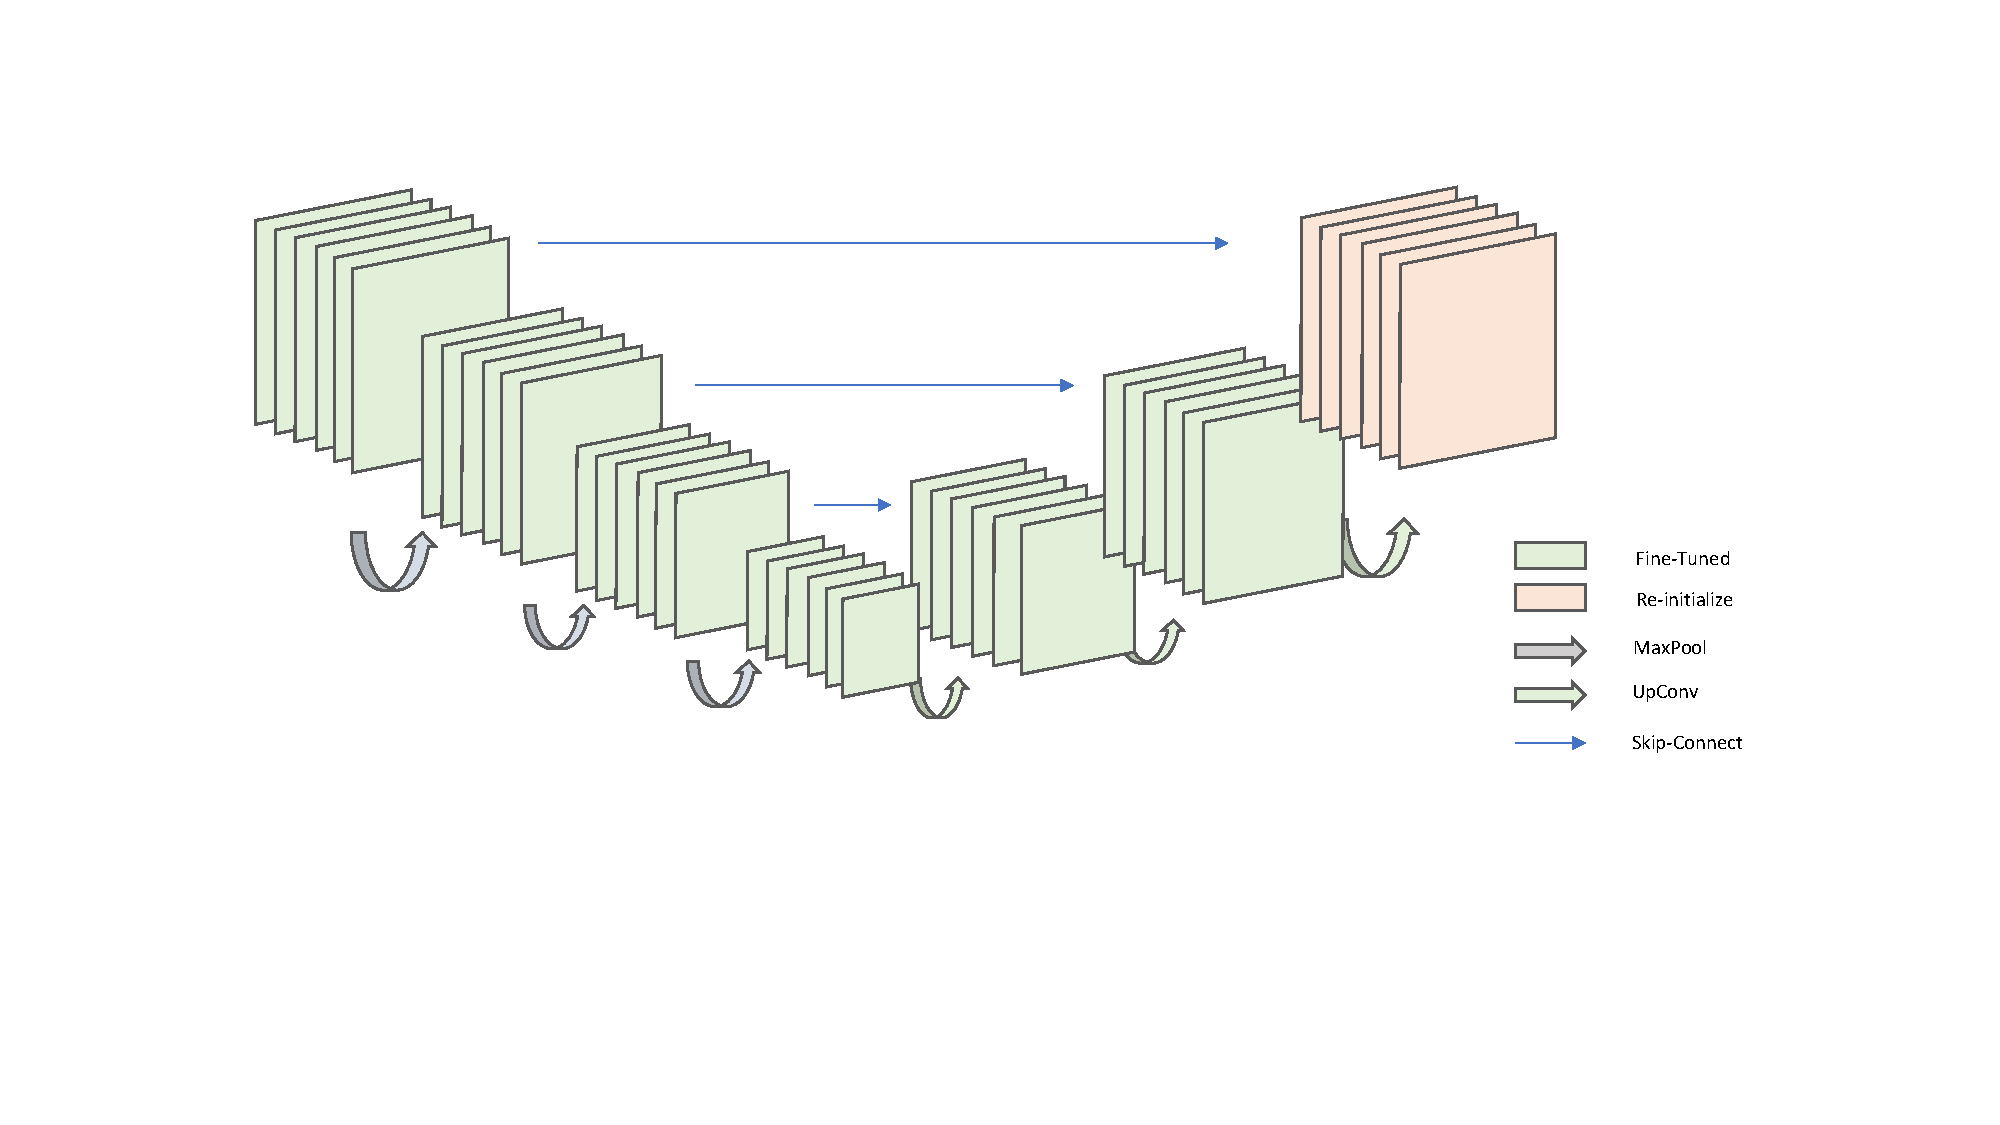
\includegraphics[width=0.8\textwidth]{img/Networks/Transfer-Finetune-all.pdf}
%	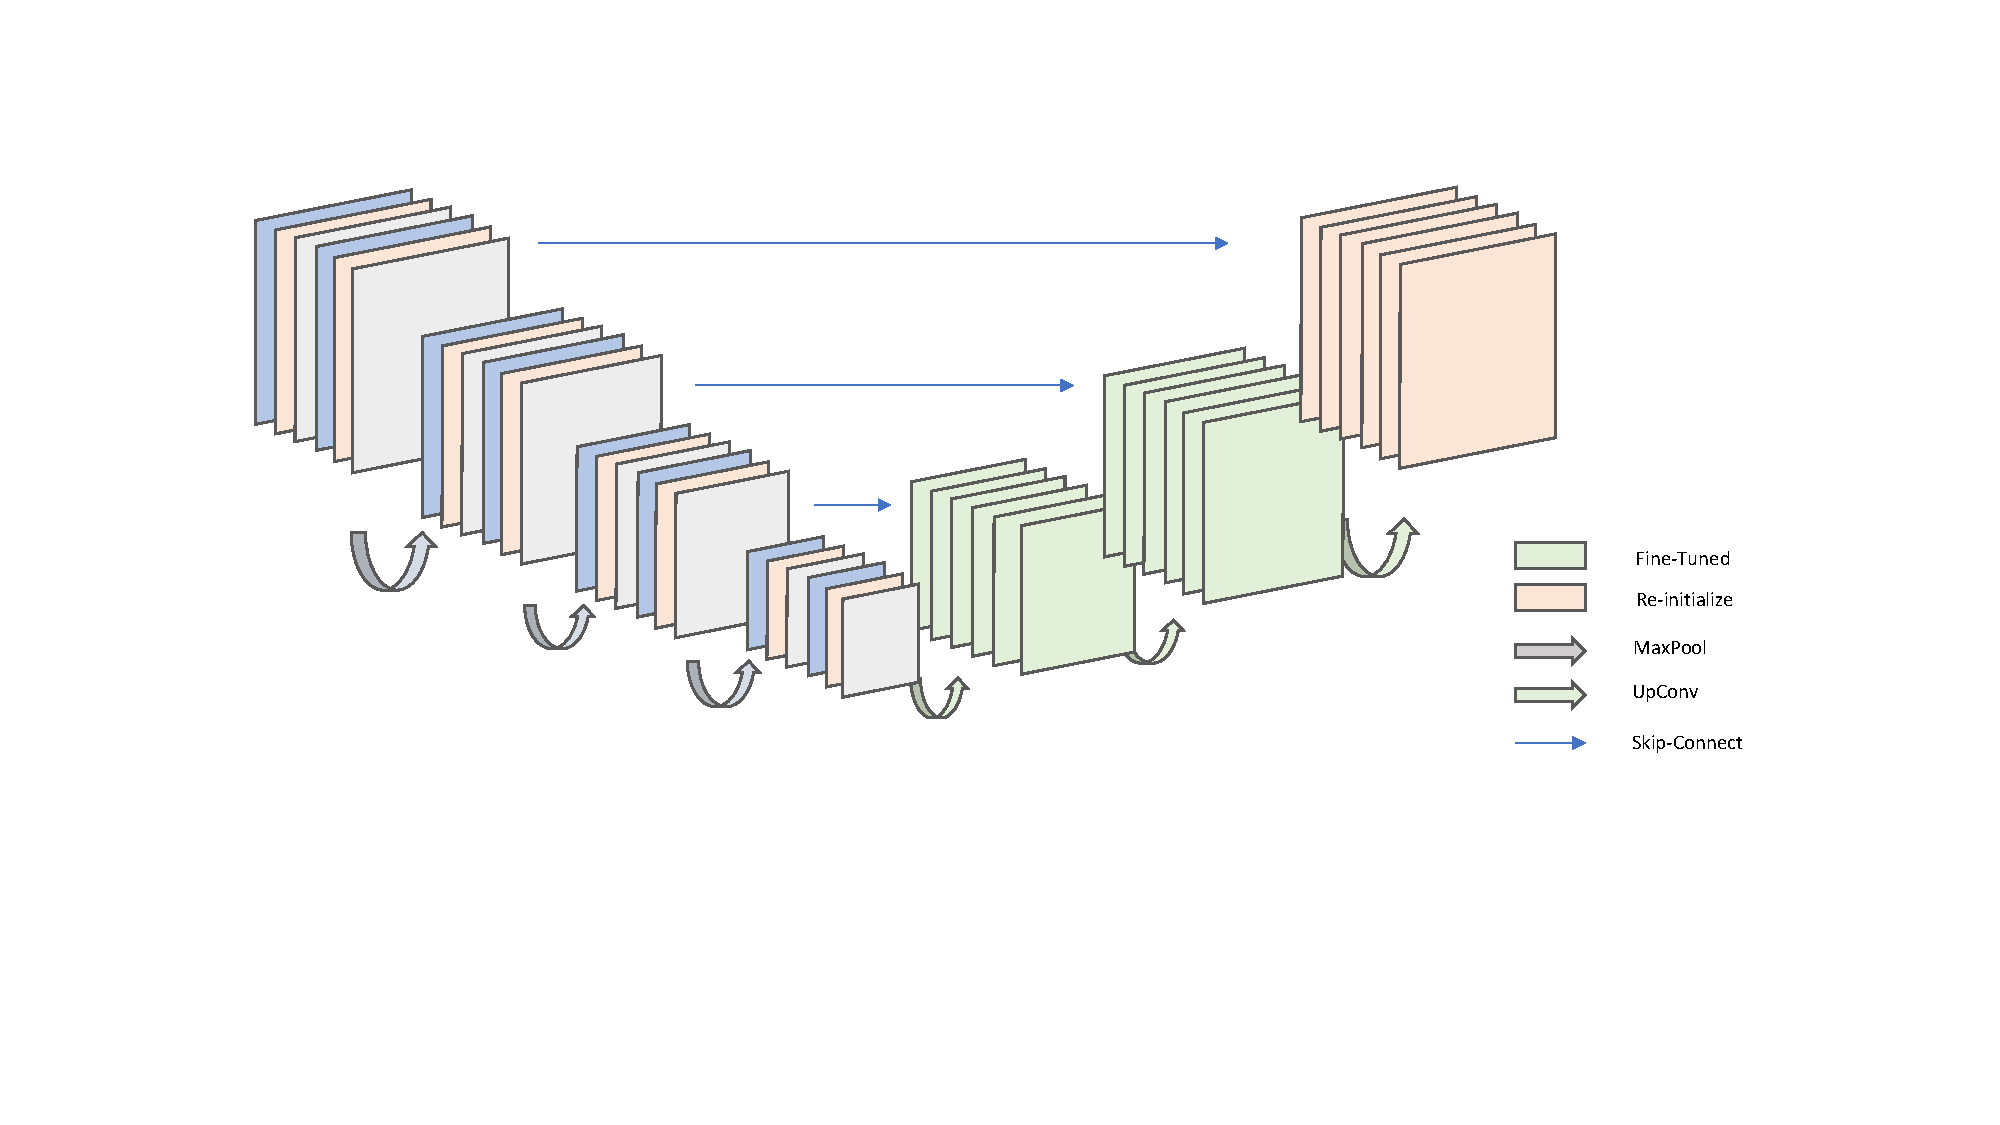
\includegraphics[width=0.8\textwidth]{img/Networks/Transfer-freeze-encoder.pdf}
%	\caption{An illustration of Network structure used for pretraining and transfer-learning}
%	\label{fig:transfer-learning-graph}
%\end{figure}
%
%\textbf{Pretraining with NSCLC and MSD Dataset}\\
%
%First the we pretrained the segmentation model using non-Covid dataset based on the assumption that the weights serves as good starting point for the fine-tuning stage. Figure \ref{fig:filtered_Lung} plots the validation loss every 10 epochs.\\
%%\begin{figure}
%%	\centering
%%	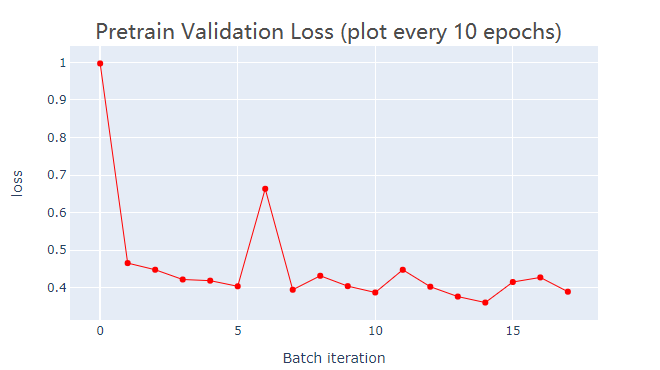
\includegraphics[width=0.8\textwidth]{img/Loss_curves/Pretrain_lungs_plot}
%%	\caption{Validation Loss with pre-training on non-Covid Lung dataset}
%%	\label{fig:pretrain_lungs}
%%\end{figure}
%
%\textbf{Fine Tuned with Model Genesis:}\\
%
%{\color{red}Paper \cite{zhou_models_2019} pretrained a 3D Unet-like model using several public dataset in the way that trained the model to restore image using destroyed image. The model was published in 3D \footnote{https://github.com/MrGiovanni/ModelsGenesis/tree/master/pytorch}. Since we did out experiment in 2D, we first load the 3D model and extract the layer weight. Then we flatten the weights into 2D as the initialization.}\\
%
%\textbf{Freezing encoder:}
%We freeze the first half of the encoder, and fine tuned the decoder except that we re-initialized the output layer.\\
%
%\textbf{Fine-Tune-All:}
%The whole network is fine tuned and the last block of convolutional layers was reinitialized. \\

\begin{table}[h]
	\centering
	\begin{tabular}{l  c c c c}
	\hline
	\hline
	Unet	&		&	Train	&	Validation	&	Test	\\
	\hline
	From Scratch	&	10-40 split	&	0.9894	&	0.7012	&	0.6893	\\
			&	40-10 split	&	0.9705	&	0.8119	&	0.8012	\\
	Fine Tune Decoder	&	10-40 split	&	0.9771	&	0.7963	&		\\
			&	40-10 split	&	0.9693	&	0	&		\\
	Fine Tune All	&	10-40 split	&	0.9802	&		&		\\
			&	40-10 split	&	0.9562	&		&		\\
	\hline
	\hline
	Attention gated Unet	&		&	Train	&	Validation	&	Test	\\
	\hline
	From Scratch	&	10-40 split	&	0.9904	&		&		\\
				&	40-10 split	&	0.9710	&		&		\\
	Fine Tune	&	10-40 split	&	0.9521	&		&		\\
				&	40-10 split	&	0.9512	&		&		\\
	Fine Tune All	&	10-40 split	&	0.9608	&		&		\\
				&	40-10 split	&	0.9611	&		&		\\	
	\hline
	\hline
	\end{tabular}
	\caption{Training with fully labeled Dataset}
	\label{tab:fully-label-result}
\end{table}
	


\subsection{SVCCA analysis on transfer learning}

\subsubsection{Network convergence during training}
We compared the convergence on each layer throughout the training process on the segmentation model. \cite{transfusion} reported that the network converged bottom up for a classification task during training. However, this is not exactly the case in our segmentation model.\\

\textbf{Network convergence with random initialization}\\

We first want to analyze the change of network layers from random initialization towards convergence using the SVCCA tool. We iterate through the dataloader and validate every 100 epochs and save the model if the result yield better performance.\\
\begin{figure}
	\centering
	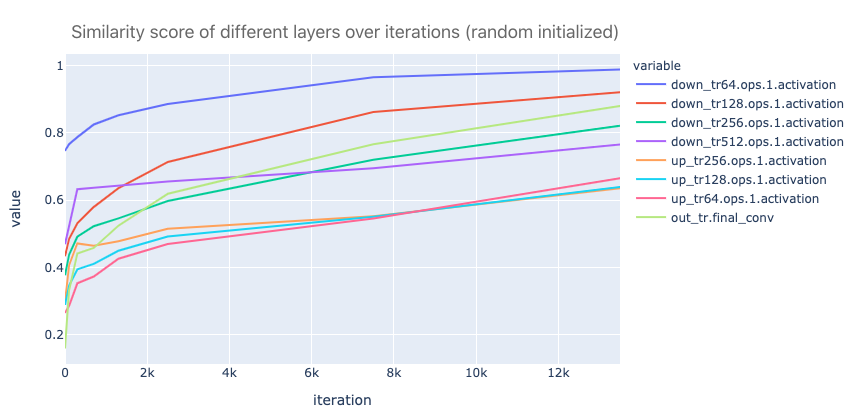
\includegraphics[width=0.8\textwidth]{img/SVCCA/CCA_score_scratch.png}
	\caption{CCA similarity score of each layer over training iterations (randomly initialized)}
	\label{fig:random_init_converge}
\end{figure}

Figure \ref{fig:random_init_converge} plots the similarity of latent space of each network layer using random initialization. 
\begin{itemize}
	\item We observed that, in general, encoder converged faster than decoder.
	\item Suprisingly, the first down convolution layer moved less comparing the initialization to the converged model.
	\item The similarity score in the output layer converged slightly faster than the other decoder part. Our explanation is that, the model performance (accuracy) increased faster in the first few number of iterations then slowly improved throughout the training.
	\item Although the similarity of the several Up-Convolution in the decoder part kept changing in the later stage of training, the output layer(out\_tr.finalconv in figure \ref{fig:random_init_converge}) did not moved much. One implication is that, Neural Network may learn different latent feature space while giving similar performance with respect to the accuracy.
\end{itemize}

\begin{figure}
	\centering
	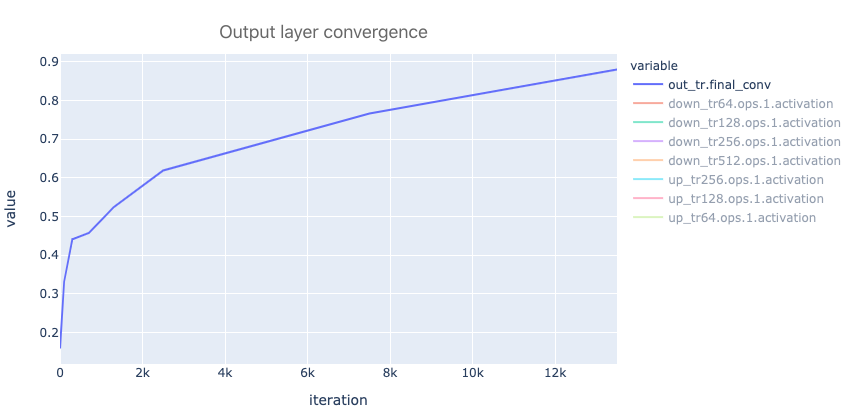
\includegraphics[width=0.8\textwidth]{img/SVCCA/from_scratch_output_layer.png}
	\caption{Filtering out the output layer convergence}
	\label{fig:random_init_converge}
\end{figure}

%\textbf{Train from scratch and transfer learning}\\
%We first compared the model before and after transfer learning. We saved the model that trained from scratch using the Covid dataset and the model pretrained using Lung dataset then fine-tuned to Covid dataset

\textbf{Network convergence during Fine-tuning}\\

The question we asked is: \textbf{Is the convergence similar to random initialization when we have a pre-trained model?}
To test the convergence, we repeated the experiment in the previous section: Starting from a pre-trained model, we iterate through the Dataloader (containing 40 volumes sliced into 2D from the Axis view) and validate every 100 iterations. We saved the model of that epoch if the validation accuracy reported a better performance. Figure \ref{fig:transfer-convergence} plots the CCA similarity score of each saved model compared with the converged model.

\begin{figure}
	\centering
	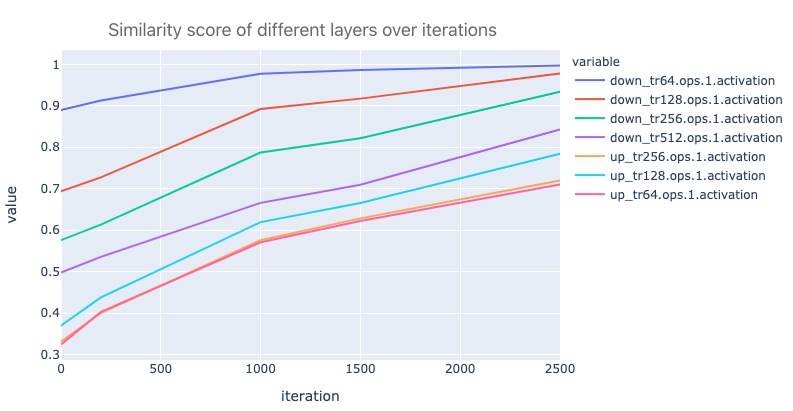
\includegraphics[width=0.8\textwidth]{img/SVCCA/CCA_score_transfer_learning}
	\caption{CCA similarity score of each layers over iterations during Fine-tuning}
	\label{fig:transfer-convergence}
\end{figure}

Comparing the similarity of feature map in the segmentation model, we observed the following behaviour:
\begin{itemize}
	\item In the Encoder part, lower layers converged faster compared to higher layers. Specifically, down covolution reported higher similarity score from the beginning compared with the similarity score obtained when we trained from scratch
	\item Layers in the Decoder observed convergence almost at the same time.
\end{itemize}

\subsubsection{Feature space comparison for transfer learning} 
%%TODO Change the title here
Another question we want to discuss is: \textbf{How much did the model move given the amount of data it observed during the Fine-Tuning?}\\

\textbf{A larger amounts of data:}\\
Figure \ref{fig:transfer-convergence} shows that, although all layers output seen a higher similarity score as the iteration number increase, 
Down-Convolution layers in the Encoder moved much less compared to the rest of the model, yielding a slightly better feature reuse during Fine-Tuning, and the feature reuse decreased from lower layers to higher layers. The Decoder, however, gives a much lower similarity score (lower than 0.5) comparing the pre-trained initialization to the converged model. Figure \ref{fig:layer-wise-comparison} compared the layer-wise feature space similarity which showed the similar obeservation.

\begin{figure}
	\centering
	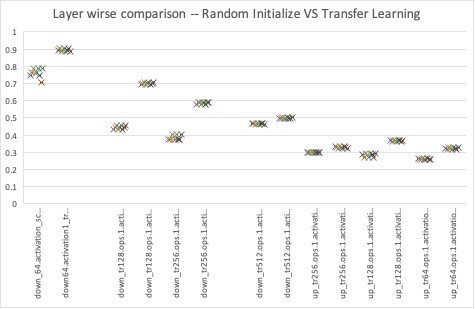
\includegraphics[width=0.8\textwidth]{img/SVCCA/randvstansfer-init2converge.png}
	\caption{Layer-wise Comparison during training}
	\label{fig:layer-wise-comparison}
\end{figure}

{\color{red}{We then trained the model using only 5 volumed sliced into 2D......}}

\section{With unlabeled data}
We then consider leveraged unlablled data because in mid July, MosMed published unlabelled CT volumes. Thus, we continued our experiment to leveraged the unlabeled dataset. 
 We first fine tune a pre-trained model on the annotated dataset, take the encoder of the network. We cropped patches from the unannotated images, assign noisy label to them and train a mean-teacher style network using those cropped patches

\subsection{Experiment Setup}
Apart from the labelled datset described in section 5.2, we downloaded 200 unlabeled volumes and first preprocessed the CT volumed as we described in chapter 3.

\subsection{Training a coarse 3D segmentation}
The purpose of leveraging unlabelled data during training is to improve the generalization of the network so that it generalize better on unseen data. We want to crop more infection area to guide the segmentation model, so we first train a coarse 3D segmentation to generate a 'rough mask' of the image to guide the segmentation.
% TODO show an example here
\subsection{Transfer learning 2D segmentation}
%TODO add sth here

\subsection{Psuedo Label Assignment -- Cosine Similarity in the feature space}
%TODO: change GAP to GMP
\begin{figure}[h]
	\centering
	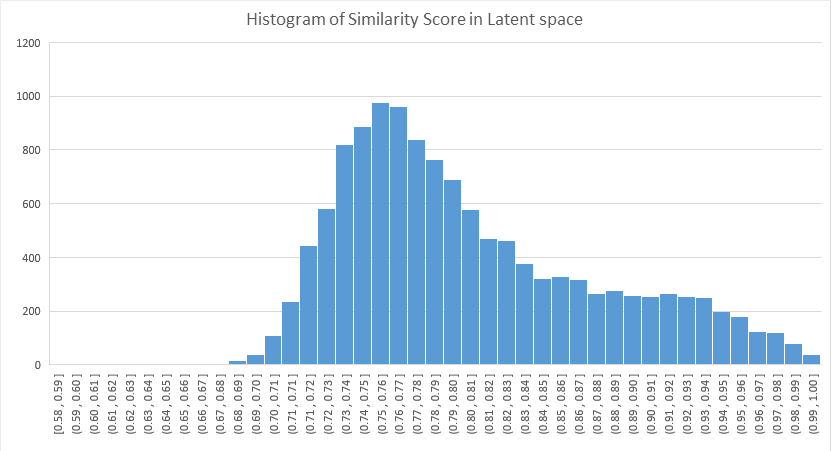
\includegraphics[width=0.8\textwidth]{img/semi-experiment/cosine_sim_histogram}
	\caption{Histogram of Cosine Similarity score}
	\label{fig:score_hist}
\end{figure}

Figure \ref{fig:score_hist} counts the occurence of similarity score over all sampled unlabeled patches. We took those samples with similarity score between 0.87 and 0.96 (sim $\in$ [0.87, 0.96]), and we assign the label of the annotated samples with highest similarity score. Figure \ref{fig:patches_noisy_mask} showed some examples of noisy labels assigned using this method.	

\begin{figure}[h]
	\centering
	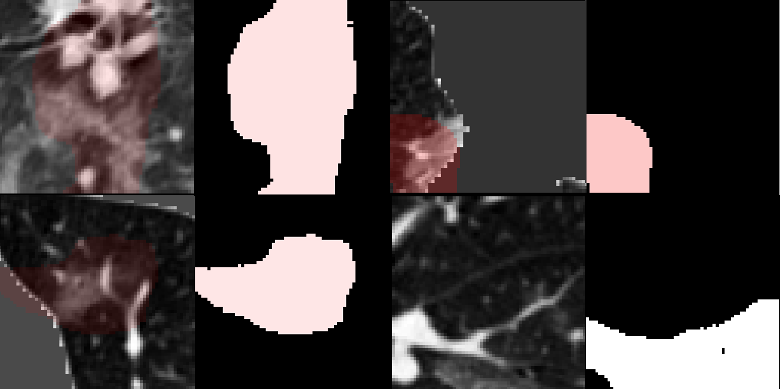
\includegraphics[width=0.8\textwidth]{img/semi-experiment/fake_assign_example}
	\caption{Example patches and noisy masks}
	\label{fig:patches_noisy_mask}
\end{figure}
\subsection{Mean teacher training}


